\section{Limits on anomalous quartic couplings} %\subsection{Limits without a Form Factor}
\label{sec:limits_pT}

The photon $E_T$ distribution is used as an observable to set limits on
the anomalous coupling parameters. Following the application
of all selection criteria, the photon $E_T$ distributions for data, the total background, and the individual signal models
for the muon and electron channels are binned over the range 30-450 GeV. Example photon $E_T$ distributions for muon and electron 
channels are shown in Fig.~\ref{photonplots}, along with the predicted signal from
WW$\gamma\gamma$ AQGC for $a_{0}^{W}/\Lambda^{2} = 50~$TeV$^{-2}$. The last bin includes the overflow.

\begin{figure}[htb]
   \begin{center}
  \subfigure[]{
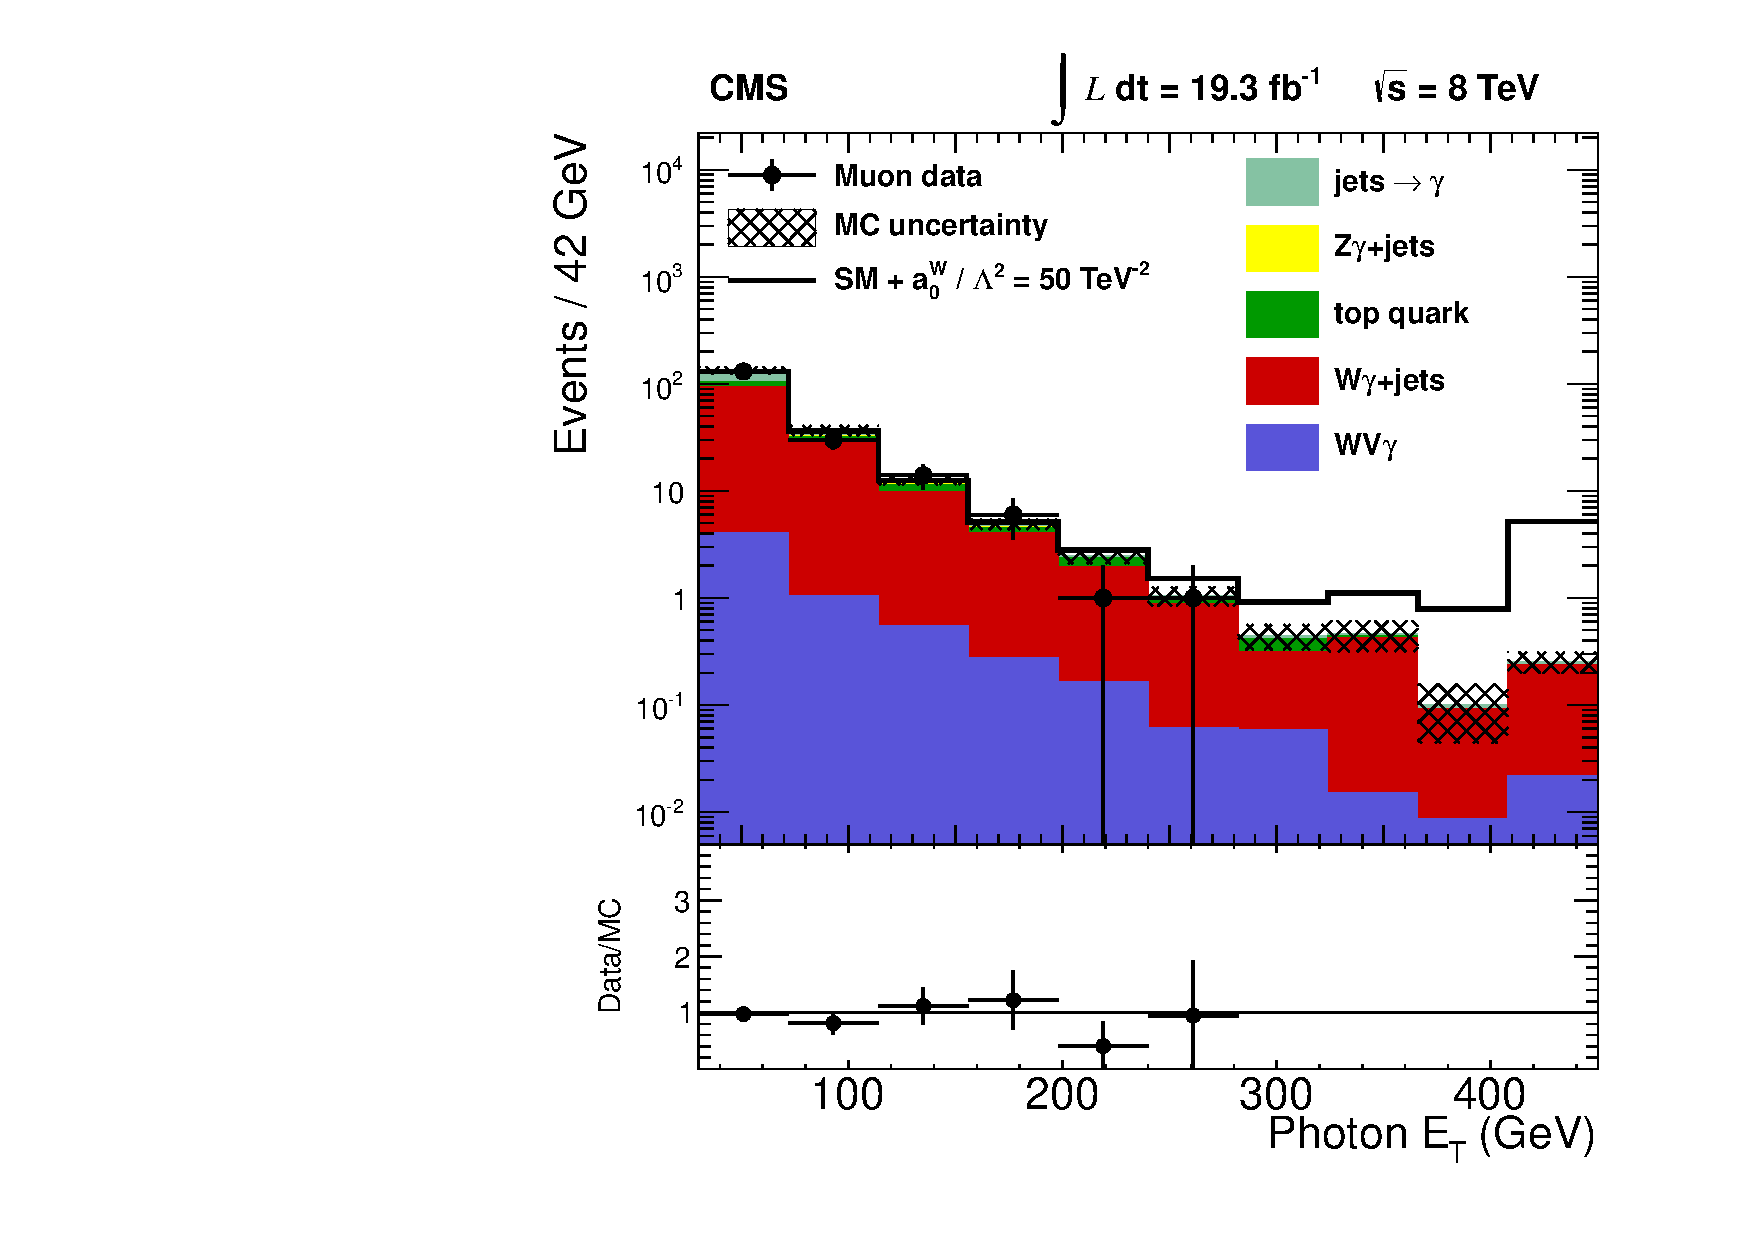
\includegraphics[width=.51\textwidth]{figs/mu_Photon_et_aQGC_log.pdf} }
  \subfigure[]{
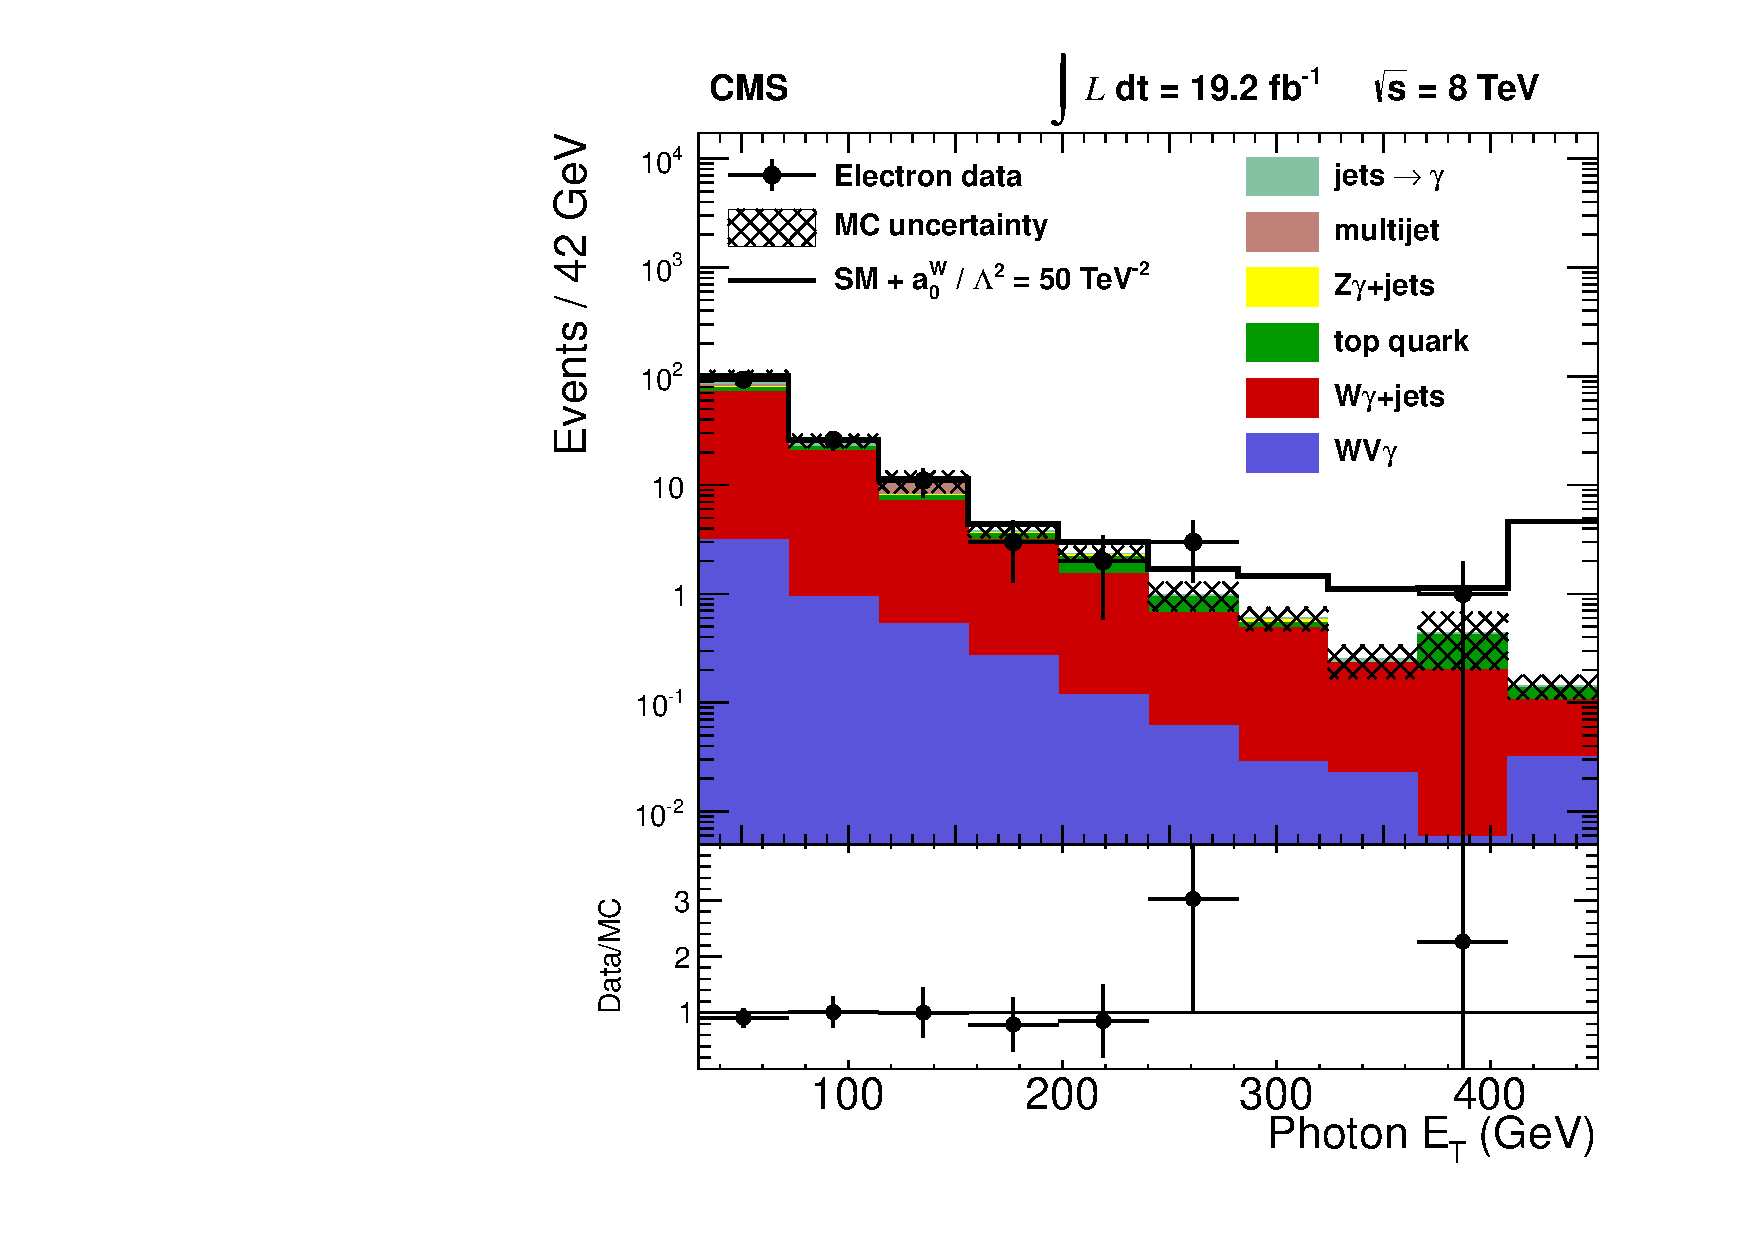
\includegraphics[width=.51\textwidth]{figs/el_Photon_et_aQGC_log.pdf}

} \caption{Comparison between predicted and observed photon $E_T$
distribution in the (a) muon and (b) electron channels. The rightmost bin
includes the integral of events above 450~GeV for each process.The solid black
line depicts a representative signal distribution with anomalous coupling parameter
$a_{0}^{W}/\Lambda^{2} = 50/$TeV$^{-2}$. }
\label{photonplots}
\end{center}
\end{figure}

Figure~\ref{fig:limitinput} shows how the predicted photon $E_T$ distributions for signal in the muon channel vary
for several values of the AQGC parameters. The corresponding distributions for the electron channel are similar.

%The binning is
%chosen such that the left-most bin begins at the first 2012 dataset
%point, and the right-most bin begins just beyond the point where is expected at least one background
%event.

\begin{figure}[b]
  \begin{center}
   \scalebox{0.90}{
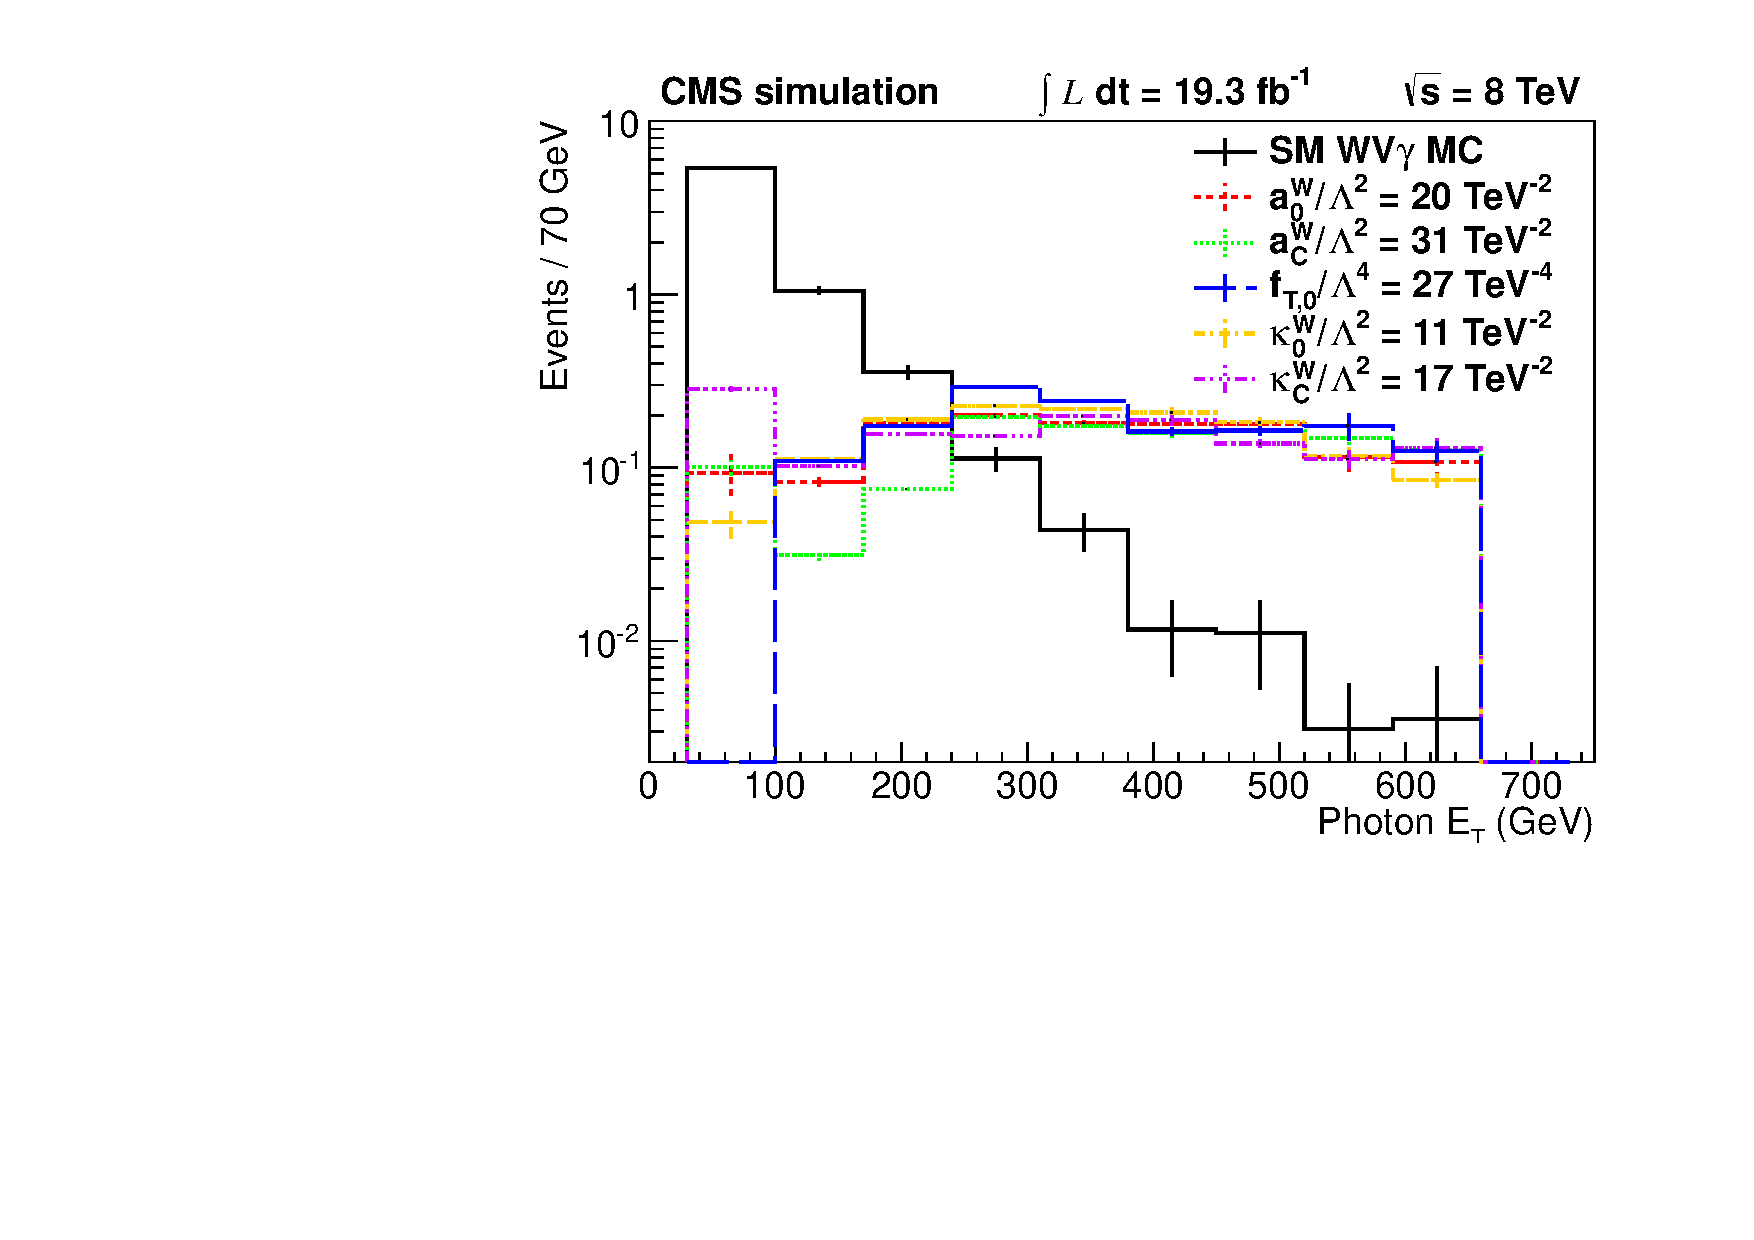
\includegraphics[width=0.75\textwidth]{figs/mu_limit_input.pdf}
   }
    \caption{ Expected photon $E_T$ distributions after the selection for the muon channel: SM prediction (black), AQGC excess from SM
prediction for $a_{0}^{W}/\Lambda^{2}$ (red), $a_{C}^{W}/\Lambda^{2}$ (green), $f_{T,0}/\Lambda^{4}$ (blue),
$\kappa_{0}^{W}/\Lambda^{2}$ (orange), and $\kappa_{C}^{W}/\Lambda^{2}$ (violet).}
    \label{fig:limitinput}
  \end{center} \end{figure}

The upper limits are set utilizing a profile likelihood asymptotic approximation method. 
Figure~\ref{fig:limitshape1d_noMVA} shows the observed and expected exclusion limits for the 
combination of muon and electron channels. Exclusion limits for
$a_{0}^{W}/\Lambda^{2}$, $a_{C}^{W}/\Lambda^{2}$,
$f_{T,0}/\Lambda^{4}$, $\kappa_{0}^{W}/\Lambda^{2}$, and
$\kappa_{C}^{W}/\Lambda^{2}$ are computed at 95\% CL, 
defined by one-tailed integrals with 5\% 
probability, and are listed in Table~\ref{tab:limit_values_noMVA}. 
%A value of zero for the AQGC parameters corresponds to the SM prediction of the QGC strength. 
Table~\ref{tab:limit_values_noMVA_dim8} contains the transformed
dimension 8 limits from the limits on the $a_{0}^{W}$ and $a_{C}^{W}$ parameters. 
%A small asymmetry in the limits is expected due to
%interference between the SM and AQGC processes.

\begin{table}[htb] 
  \caption{The 95\% CL exclusion limits for each aQCG parameter from the combination of the muon and electron channels.}
  \centering 
  \scalebox{1.10}{
  \begin{tabular}{|c|c|}
  \hline
  Observed limits (TeV$^{-2}$) & Expected limits (TeV$^{-2}$) \\
  \hline
  \hline
  -21 $<$ $a_{0}^{W}/\Lambda^{2}$ $<$ 20   & -24  $<$ $a_{0}^{W}/\Lambda^{2}$ $<$ 23  \\
  -34 $<$ $a_{C}^{W}/\Lambda^{2}$ $<$ 32   & -37  $<$ $a_{C}^{W}/\Lambda^{2}$ $<$ 34  \\
  -25 $<$ $f_{T,0}/\Lambda^{4}$ $<$ 24 (TeV$^{-4}$)  & -27  $<$ $f_{T,0}/\Lambda^{4}$ $<$ 27 (TeV$^{-4}$) \\
  -12 $<$ $\kappa_{0}^{W}/\Lambda^{2}$ $<$ 10  & -12  $<$ $\kappa_{0}^{W}/\Lambda^{2}$ $<$ 12  \\
  -18 $<$ $\kappa_{C}^{W}/\Lambda^{2}$ $<$ 17  & -19  $<$ $\kappa_{C}^{W}/\Lambda^{2}$ $<$ 18  \\
  \hline
  \end{tabular}}
  \label{tab:limit_values_noMVA} \end{table}

\begin{table}[htb] 
 \centering 
  \caption{The 95\% CL exclusion limits for each dimension 8 aQCG parameter from the combination of the muon and electron channels.}
  \scalebox{1.0}{
  \begin{tabular}{|c|c|}
  \hline
  Observed limits (TeV$^{-4}$) & Expected limits (TeV$^{-4}$) \\
  \hline
  \hline
  -77  $<$ $f_{M,0}/\Lambda^{4}$ $<$ 81  & -89  $<$ $f_{M,0}/\Lambda^{4}$ $<$ 93  \\
  -131 $<$ $f_{M,1}/\Lambda^{4}$ $<$ 123 & -143 $<$ $f_{M,1}/\Lambda^{4}$ $<$ 131 \\
  -39  $<$ $f_{M,2}/\Lambda^{4}$ $<$ 40  & -44  $<$ $f_{M,2}/\Lambda^{4}$ $<$ 46  \\
  -66  $<$ $f_{M,3}/\Lambda^{4}$ $<$ 62  & -71  $<$ $f_{M,3}/\Lambda^{4}$ $<$ 66  \\
  \hline
  \end{tabular}}
  \label{tab:limit_values_noMVA_dim8} \end{table}


\begin{figure}[hb]
  \begin{center}
    \subfigure[]{
    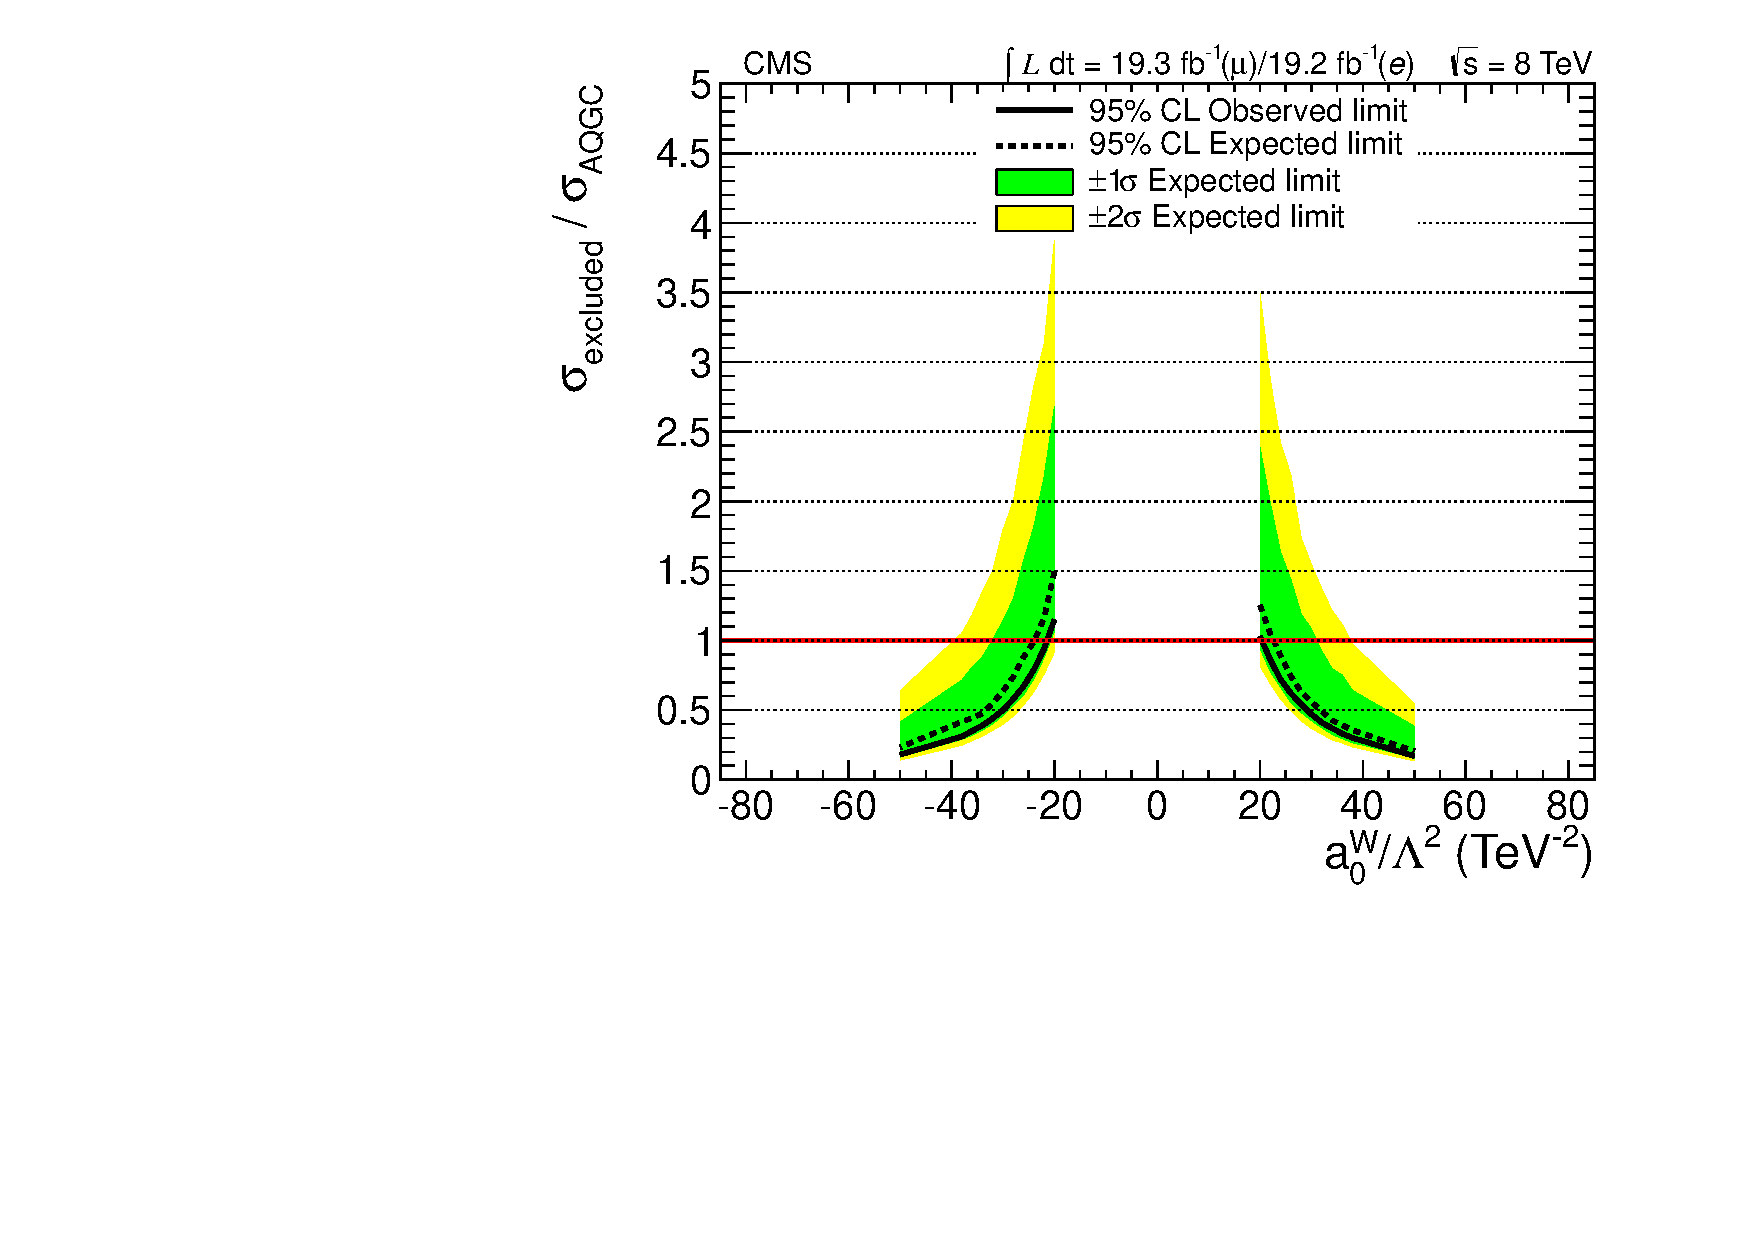
\includegraphics[width=0.49\textwidth]{figs/a0W_PhotonPT_limit_noMVA.pdf}
  }
    \subfigure[]{
    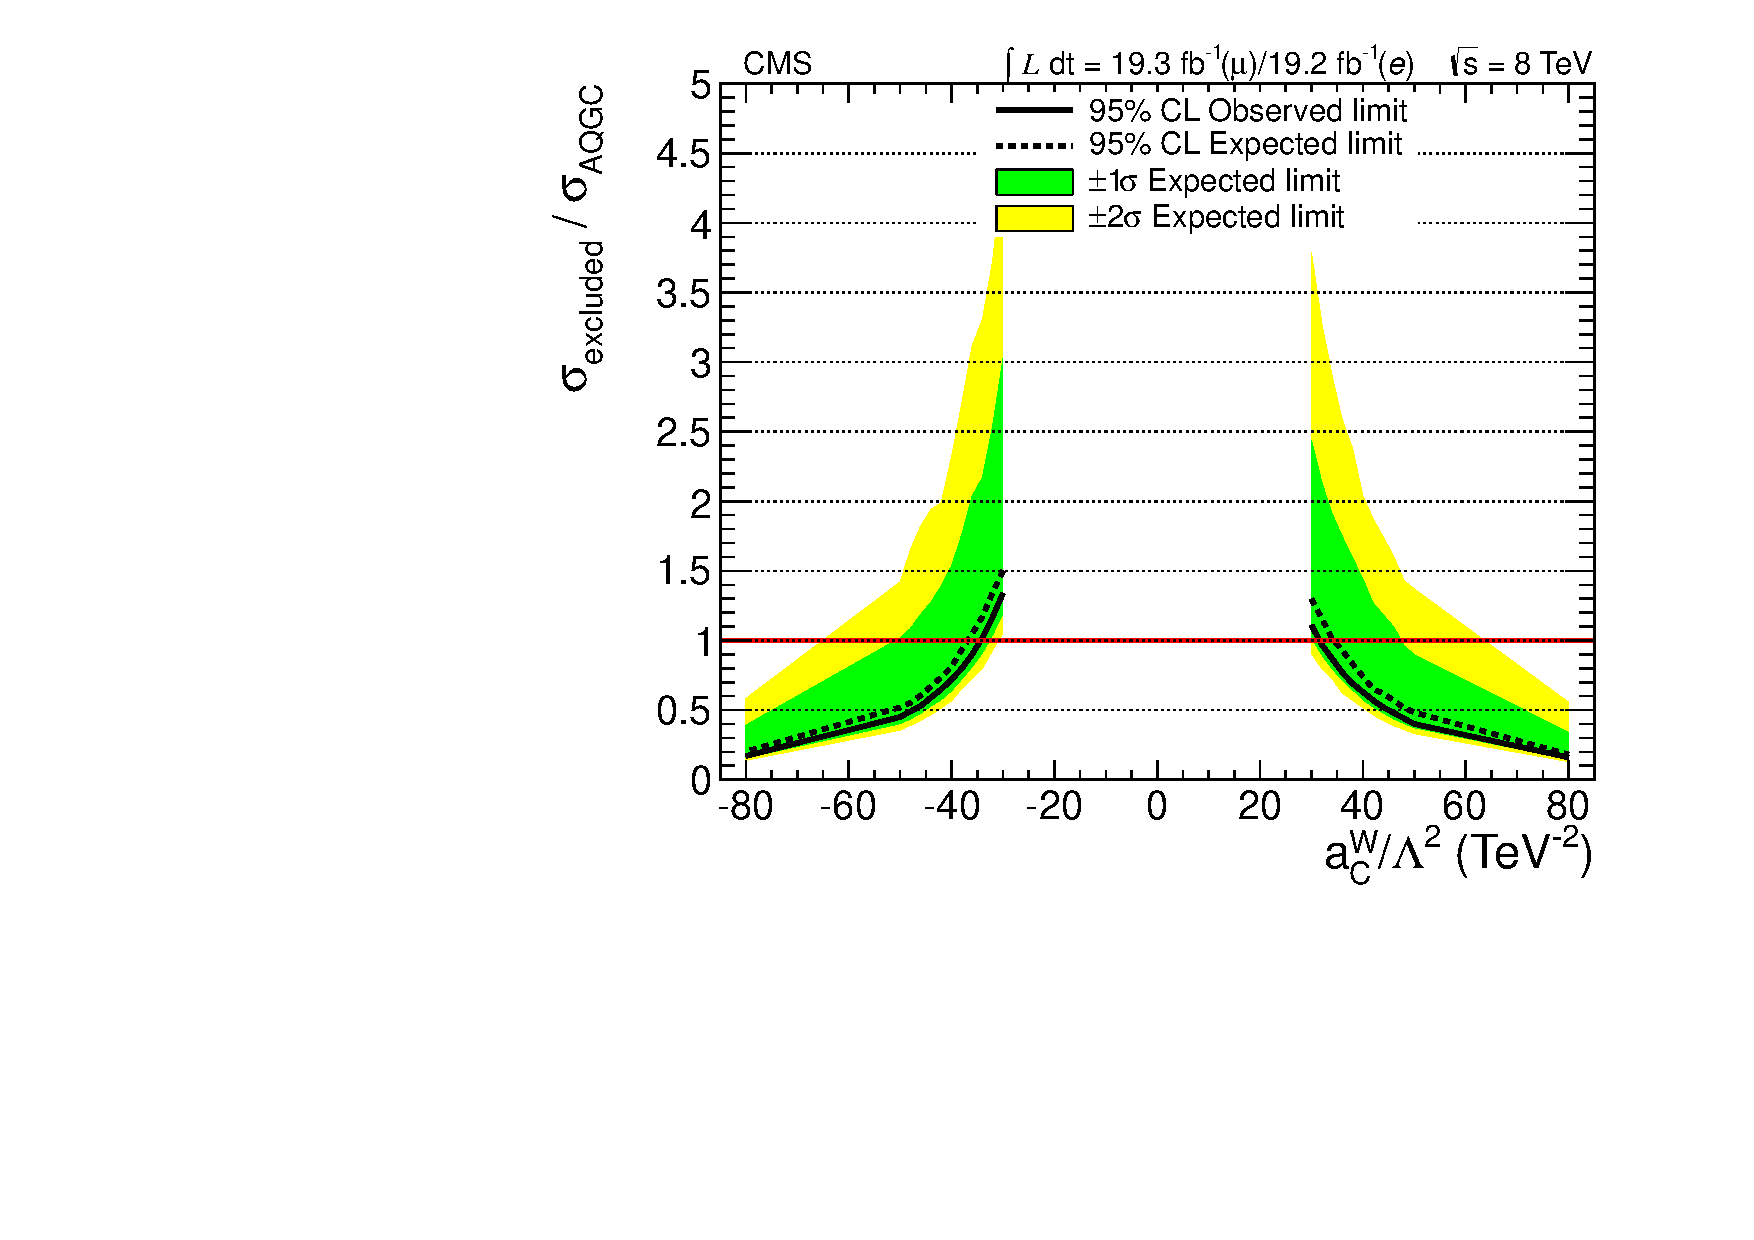
\includegraphics[width=0.49\textwidth]{figs/acW_PhotonPT_limit_noMVA.pdf}
  }\\
  \subfigure[]{
    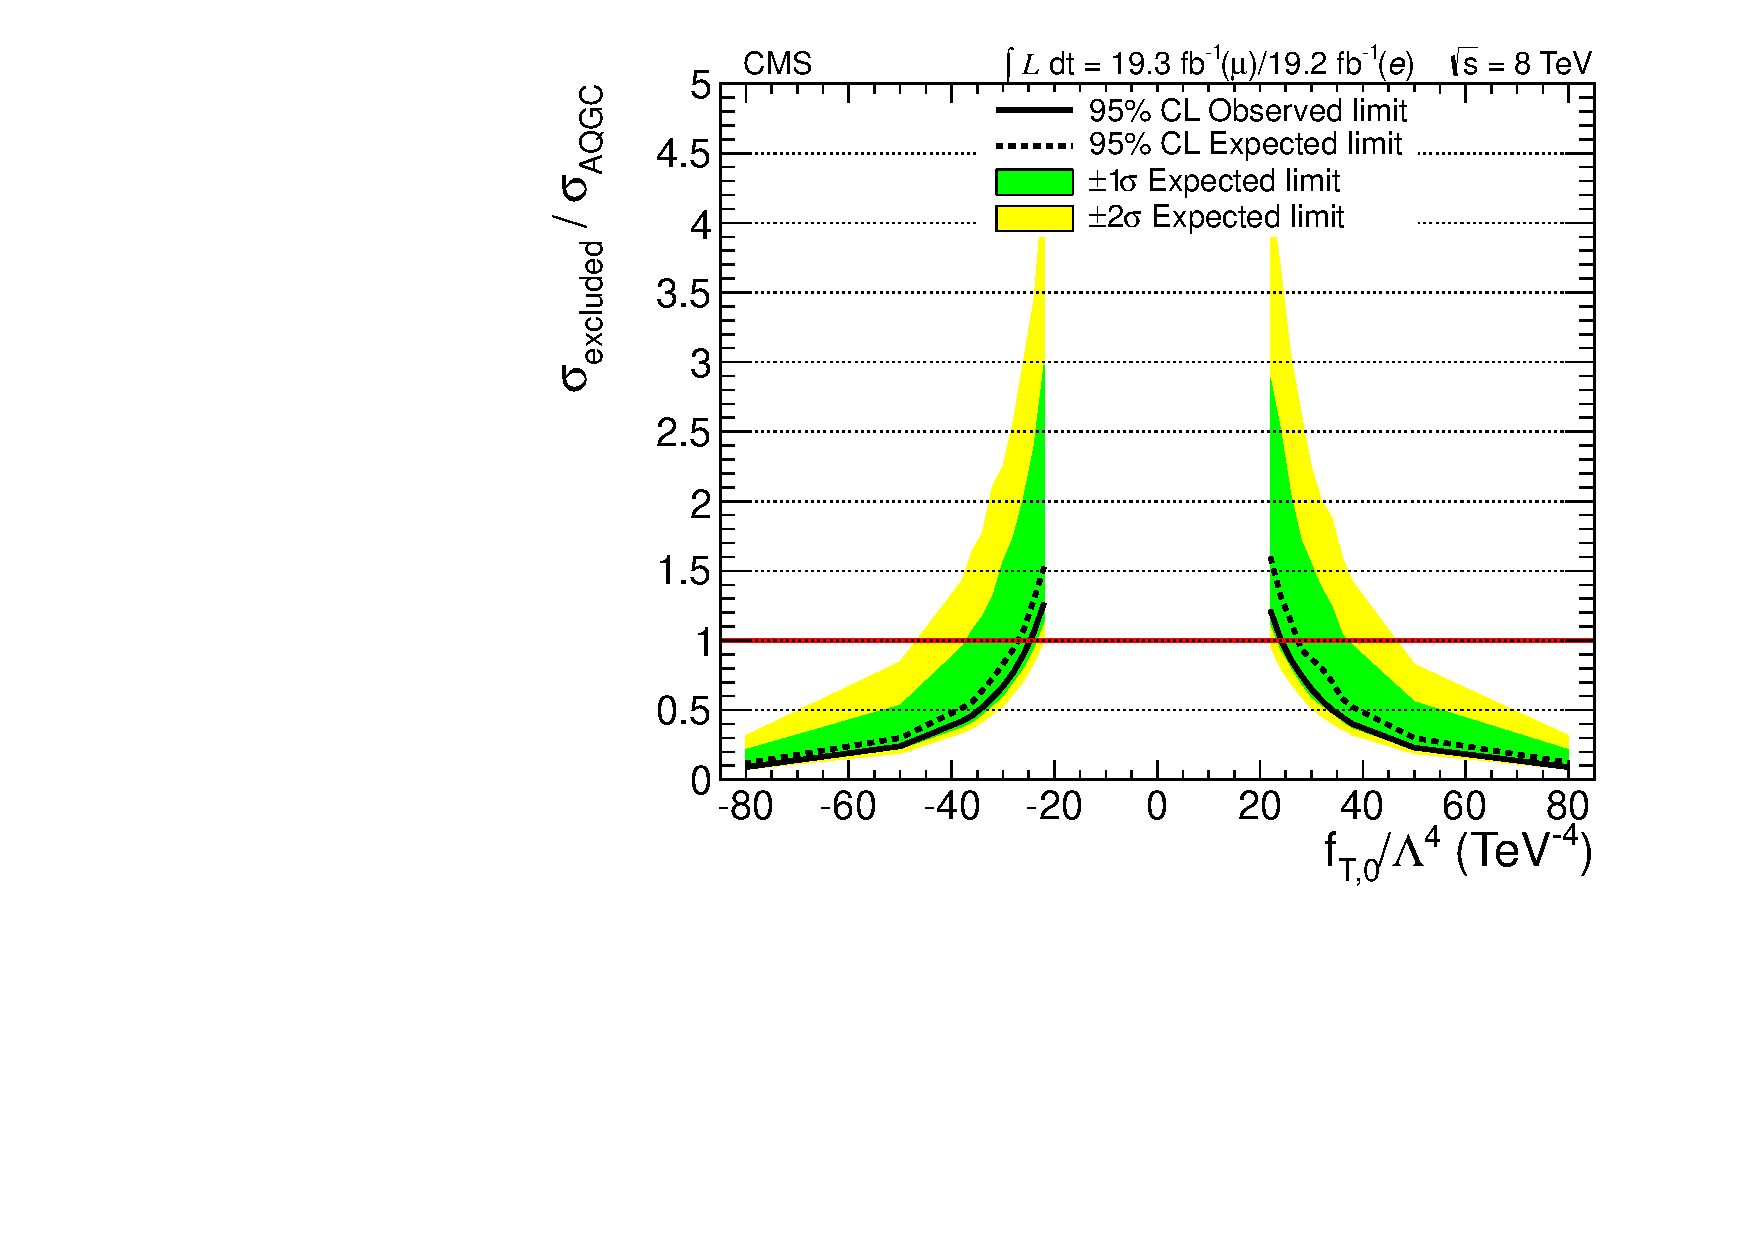
\includegraphics[width=0.49\textwidth]{figs/LT0_PhotonPT_limit_noMVA.pdf}
  }
  \subfigure[]{
    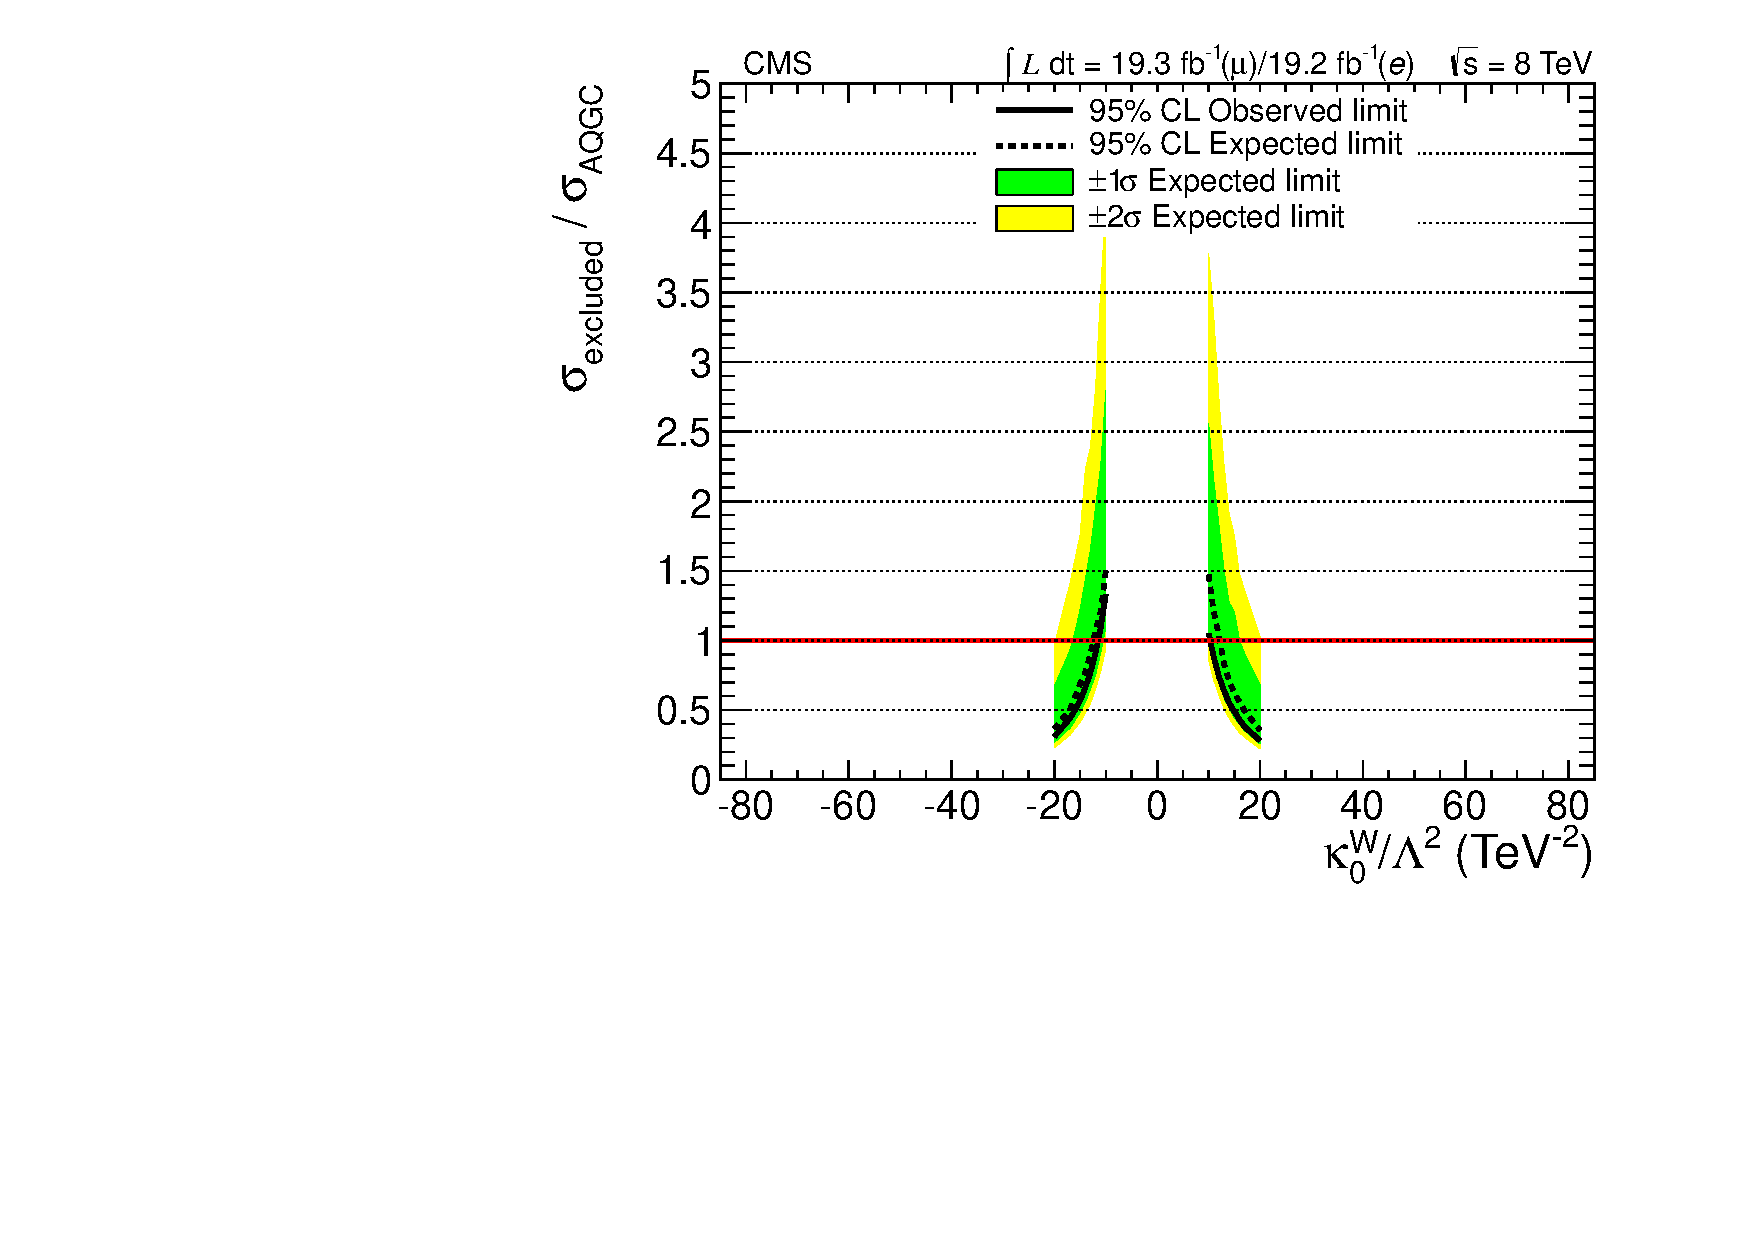
\includegraphics[width=0.49\textwidth]{figs/K0W_PhotonPT_limit_noMVA.pdf}
  }\\
  \subfigure[]{
    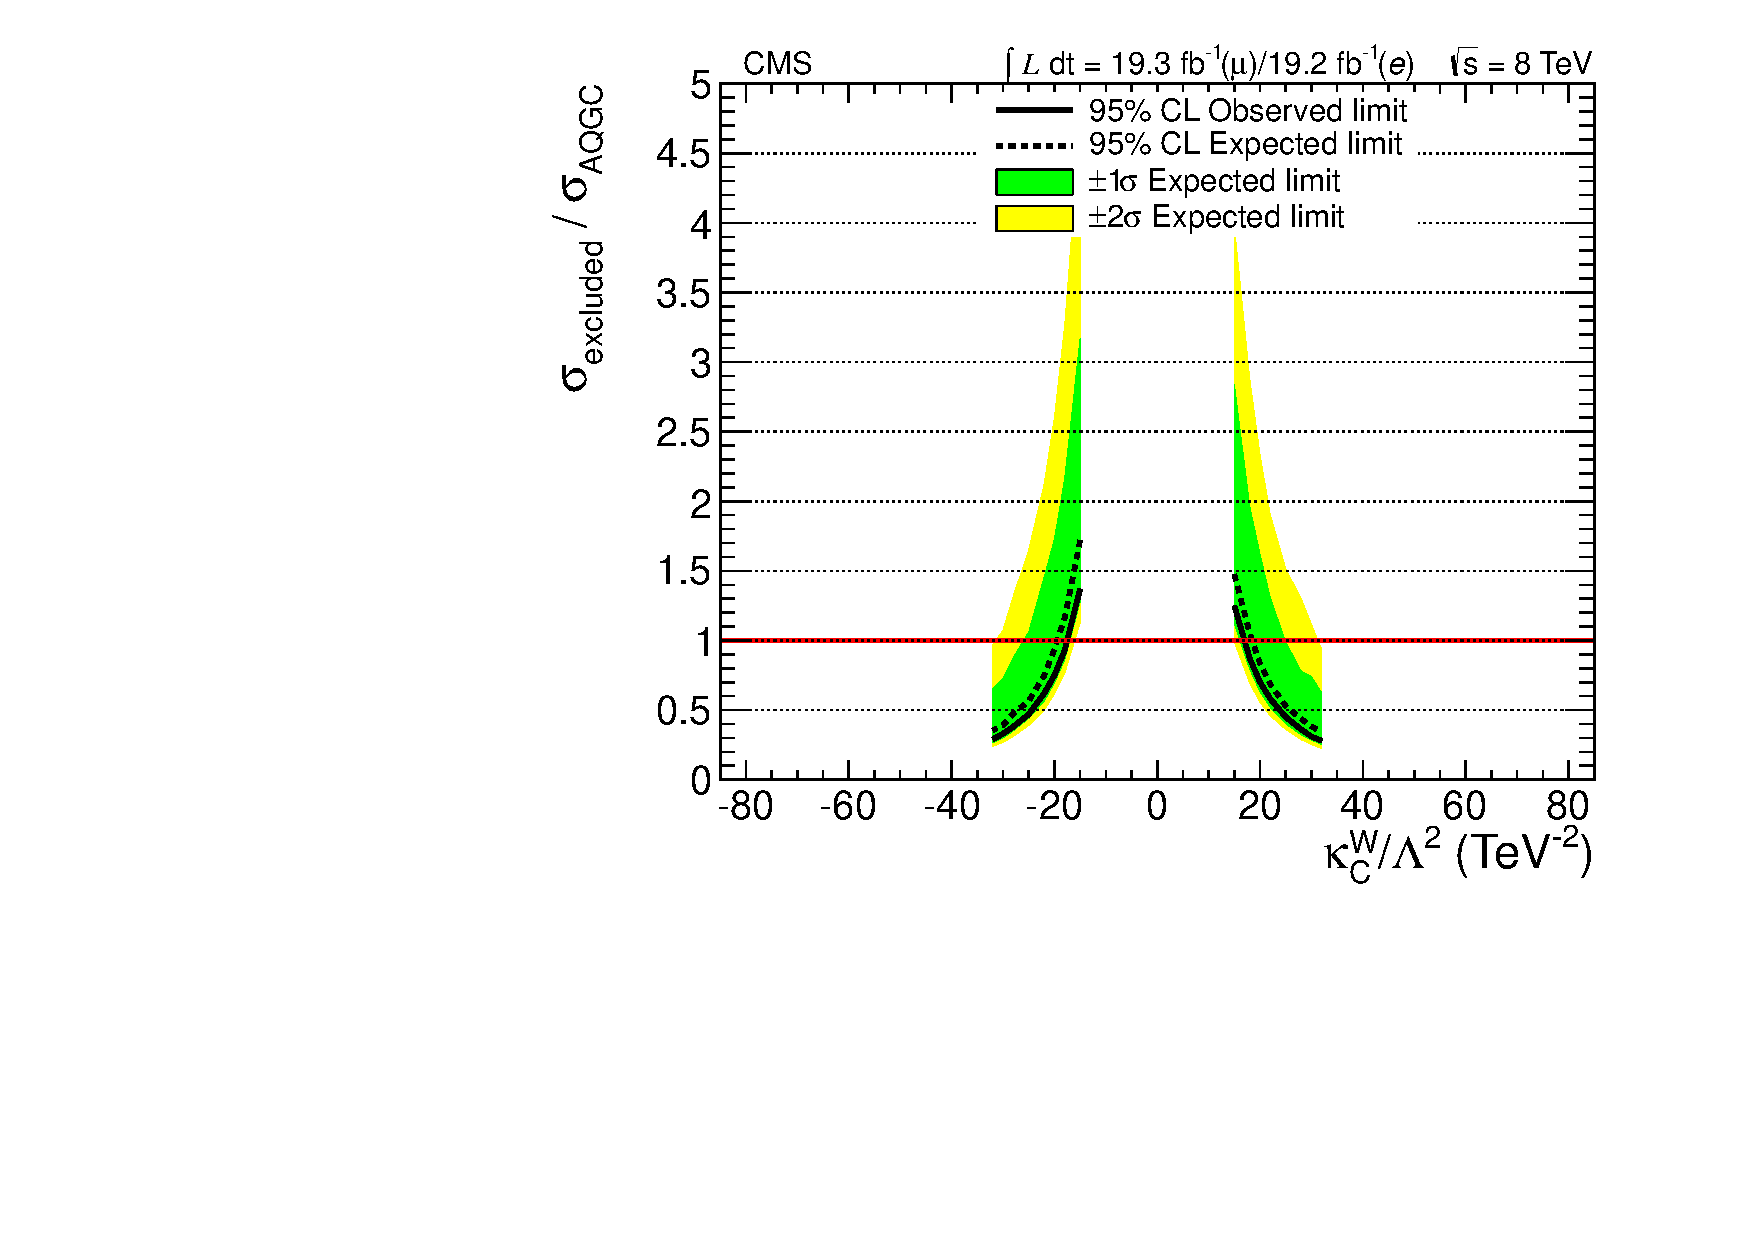
\includegraphics[width=0.49\textwidth]{figs/KCW_PhotonPT_limit_noMVA.pdf}
  } % \subfigure[]{ % 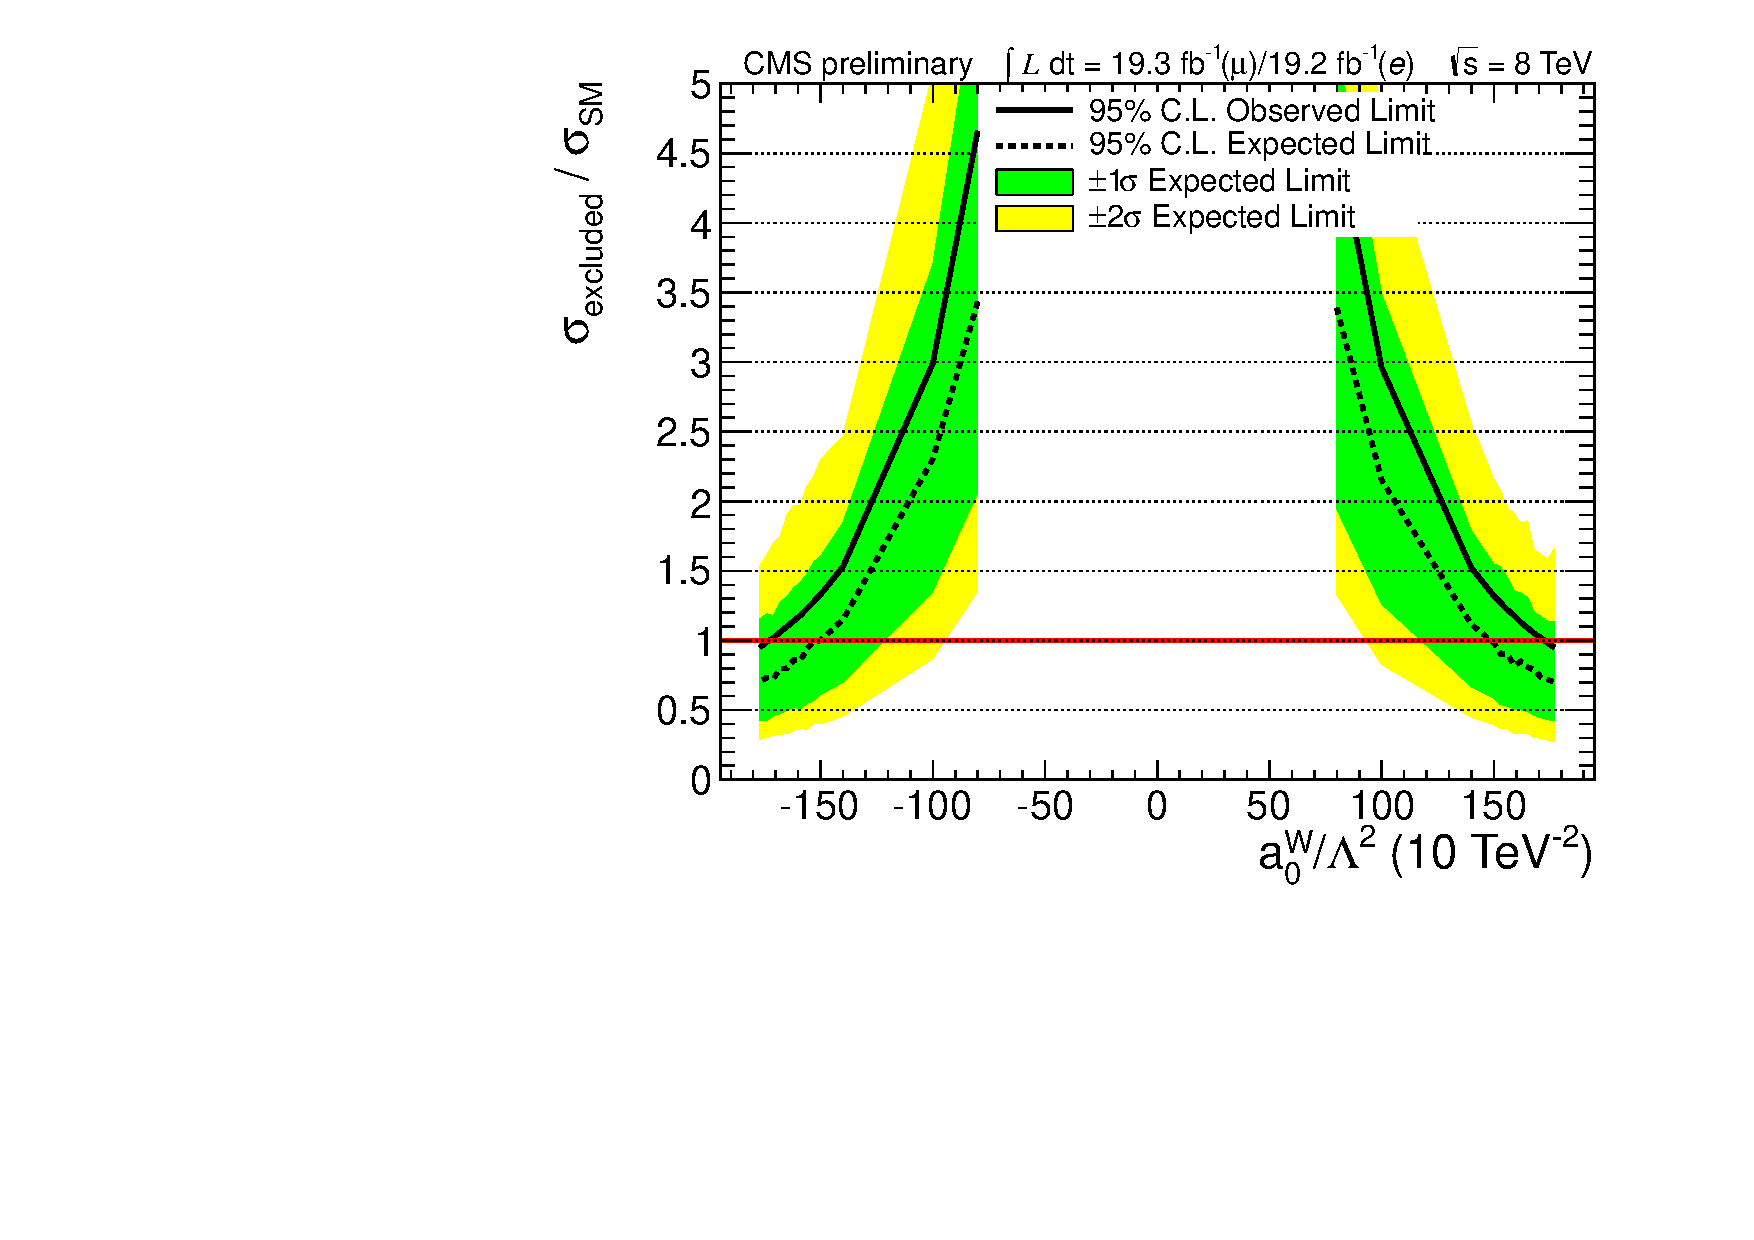
\includegraphics[width=0.45\textwidth]{figs/a0W_PhotonPT_limit_noMVA_500FFn2.pdf} % }
    \caption{ 95\% CL exclusion limits for (a) $a_{0}^{W}/\Lambda^{2}$, (b) $a_{C}^{W}/\Lambda^{2}$, (c) $f_{T,0}/\Lambda^{4}$, (d) 
$\kappa_{0}^{W}/\Lambda^{2}$, and (e) $\kappa_{C}^{W}/\Lambda^{2}$.}
    \label{fig:limitshape1d_noMVA}
  \end{center} \end{figure}

A comparison of several existing limits on the WW$\gamma\gamma$ AQGC parameter is shown in Fig.~\ref{fig:WWAAcomparison}. The CMS 
limits are orders of magnitude more stringent than the best limits obtained at LEP and Tevatron and are probing for new physics at the TeV scale.

\begin{figure}[htb] \begin{center}
   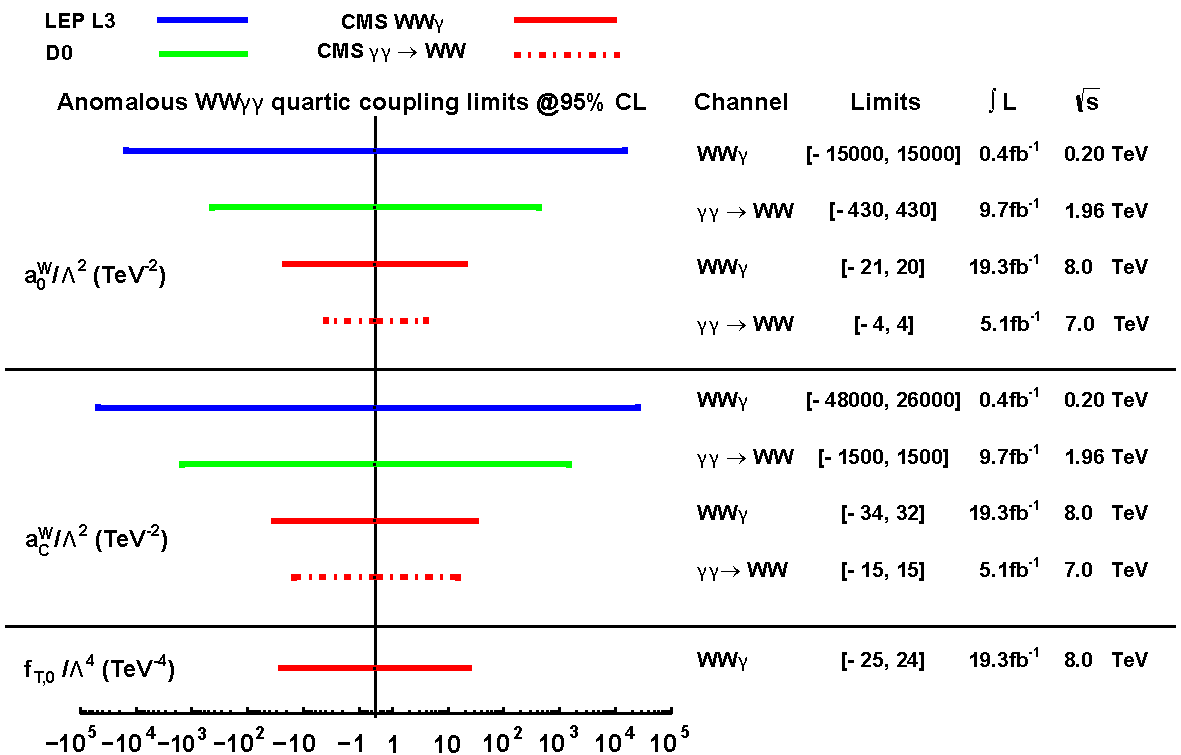
\includegraphics[width=.98\textwidth]{figs/WWaa_comparison.pdf} 
   \caption{ Comparison of the limits on the WW$\gamma\gamma$ AQGC parameter obtained
from this study, together with results from exclusive $\gamma\gamma\rightarrow$WW production at CMS~\cite{Chatrchyan:2013foa} and results from the 
L3~\cite{Achard:2001eg} and the D0~\cite{Abazov:2013opa} collaborations. All liimits on AQGC are calculated without a form 
factor. } 
\label{fig:WWAAcomparison} 
\end{center} 
\end{figure}

